%%
%% copyright quintard julien
%% 
%% kaneton
%% 
%% k3-subject.tex
%% 
%% path          /root/data/research/projects/svn/kaneton/projects/k3
%% 
%% made by mycure
%%         quintard julien   [quinta_j@epita.fr]
%% 
%% started on    Mon Feb 21 16:02:38 2005   mycure
%% last update   Mon Feb 21 16:02:39 2005   mycure
%%

\documentclass[10pt,a4wide]{article}
\usepackage[english]{babel}
\usepackage{a4wide}
\usepackage{graphicx}
\usepackage{graphics}
\usepackage{fancyheadings}
\pagestyle{fancy}

\bibliographystyle{plain}

\lhead{{\scriptsize kaneton project}}
\rhead{k3 subject}
\rfoot{\scriptsize EPITA System Lab}

\title{kaneton3}

\author{Julien Quintard - \small{quinta\_j@epita.fr} \\
        Jean-Pascal Billaud - \small{billau\_j@epita.fr} \\ \\
	\small{last updated by} \\
	Julien Quintard - \small{quinta\_j@epita.fr}}

\date{\today}

\begin{document}
\maketitle

\section{Informations}

\begin{tabular}{p{7cm}l}

Date de rendu: & Lundi 14 Mars 2005 \`a 23h42 \\
Dur\'ee du projet: & 3 semaines \\
Nom du fichier de rendu: & k3.tar.gz \\
Responsable du projet: & Julien Quintard - \small{quinta\_j@epita.fr} \\
                       & Jean-Pascal Billaud - \small{billau\_j@epita.fr} \\
Newsgroups d\'edi\'es: & epita.kaneton, epita.adm.sr \\
Langages: & asm, C \\
Architectures: & Intel 32-bit \\
Nombre de personnes par groupes: & 3 \`a 5

\end{tabular}

\section{Introduction}

\paragraph{}

Votre kernel poss\`ede un gestionnaire de m\'emoire physique, une interface
de gestion des traps et des segments. D'autre part, vous communiquez
\`a pr\'esent avec des p\'eriph\'eriques basiques.

\paragraph{}

Le but de ce projet est de r\'ealiser un ensemble de fonctions pour la
gestion de la m\'emoire virtuelle.

\paragraph{}

Pour le moment le kernel dispose de son espace d'adressage virtuel.
N\'eanmoins, mis \`a part l'installation de son adressage, nous n'avons
fourni aucune interface pour ajouter, modifier ou enlever des \'el\'ements
de cet espace d'adressage.

\paragraph{}

Au terme de cette \'etape, kaneton sera capable de r\'eserver et
de lib\'erer des pages virtuelles mais \'egalement d'accomplir des t\^aches
plus complexes sur la m\'emoire virtuelle.

\section{Travail Demand\'e}

\paragraph{}

Le projet consiste \`a d\'evelopper un gestionnaire de m\'emoire virtuelle.

\paragraph{}

Il ne vous sera rien demander d'autre que le fait de fournir une interface
fonctionnelle.

\section{Interfaces}

\subsection{Espaces d'adressage virtuels}

\paragraph{}

Un espace d'adressage virtuel est un ensemble d'\'el\'ements d\'ecrivant
la m\'emoire virtuelle en mettant en relation des zones virtuelles avec des
zones physiques.

\paragraph{}

Dans le cas du processeur Intel, la m\'emoire virtuelle est d\'ecrite
par le syst\`eme de traduction d'adresses nomm\'e ``Paging'' mais
vous pourriez tout \`a fait d\'ecrire l'espace virtuel avec une structure
de donn\'ees software, \'evitant ainsi les appels \`a la couche ``machine
dependent''.

\paragraph{}

Les fonctions de gestion d'espace d'adressage: \textbf{asid\_rsv}(),
\textbf{asid\_rel}() etc.. doivent d\'esormais s'occuper de la mise en
place des structures de donn\'ees pour la gestion de la m\'emoire, physique
et virtuelle d'un processus.

\paragraph{}

Votre travail va donc \^etre de modifier les fonctions de gestion des
espaces d'adressage. Attention, ces fonctions devront \^etre compos\'ees
de deux parties. La premi\`ere partie ``machine independant'' se contentena
de g\'erer des structures de donn\'ees software alors que le seconde partie
s'occupera de la gestion des op\'erations sur les structures hardware.

\subsection{M\'emoire virtuelle}

\paragraph{}

Dans un premier temps, il vous faudra initialiser les zones virtuelles
de votre kernel.

\paragraph{}

En effet dans le bootloader, vous mappiez nombre de pages physiques
mais vous ne gardiez aucune trace de ces allocations. Pour initialiser
ce syst\`eme de trace d'allocation, prenez exemple sur votre
initialisation des zones physiques.

\paragraph{}

Votre gestionnaire de m\'emoire virtuelle doit fournir un certain nombre
de fonctionnalit\'es permettant d'allouer, de lib\'erer des pages
virtuelles mais \'egalement de manipuler des donn\'ees en virtuel.

\paragraph{}

\hspace{1.5cm}int \textbf{vm\_rsv}(t\_asid \textbf{asid},
                                   t\_vaddr \textbf{*vaddr},
                                   u\_int32\_t \textbf{npages},
                                   u\_int8\_t \textbf{flags});

\paragraph{}

Cette fonction se contente d'allouer un nombre donn\'e de pages virtuelles
dans un espace d'adressage donn\'e: \textbf{asid}. Le param\`etre
\textbf{*vaddr} est rempli par la fonction pour indiquer l'endroit ou
l'allocation a pris effet. L'argument \textbf{flags} a la m\^eme fonction
que pour la fonction \textbf{pm\_rsv}().

\paragraph{}

\hspace{1.5cm}int \textbf{vm\_rel}(t\_asid \textbf{asid},
                                   t\_vaddr \textbf{vaddr},
                                   u\_int32\_t \textbf{npages});

\paragraph{}

Cette fonction lib\`ere de la m\'emoire virtuelle.

\paragraph{}

\hspace{1.5cm}int \textbf{vm\_map}(t\_asid \textbf{asid},
				   t\_paddr \textbf{paddr},
                                   t\_vaddr \textbf{vaddr},
                                   u\_int32\_t \textbf{npages});

\paragraph{}

Cette fonction \'etablie une correspondance entre l'adresse physique
\textbf{paddr} et l'adresse virtuelle \textbf{vaddr} et cela pour
un nombre de pages donn\'e.

\paragraph{}

\hspace{1.5cm}int \textbf{vm\_unmap}(t\_asid \textbf{asid},
                                     t\_vaddr \textbf{vaddr},
                                     u\_int32\_t \textbf{npages});

\paragraph{}

Cette fonction enl\`eve la correspondance pr\'ec\'edemment
attribu\'ee.

\paragraph{}

\hspace{1.5cm}int \textbf{vm\_copy}(t\_asid \textbf{from},
                                    t\_vaddr \textbf{src},
                                    t\_asid \textbf{to},
                                    t\_vaddr \textbf{dst},
                                    u\_int32\_t \textbf{nbytes});

\paragraph{}

Cette fonction se charge de copier un nombre d'octets donn\'e entre
deux espaces d'adressage virtuels.

\paragraph{}

\hspace{1.5cm}int \textbf{mm\_rsv}(t\_asid \textbf{asid},
                                   t\_vaddr \textbf{*vaddr},
                                   u\_int32\_t \textbf{npages}
                                   u\_int8\_t \textbf{flags});

\paragraph{}

La fonction \textbf{mm\_rsv} sera charg\'ee d'allouer \textbf{npages} physiques
et virtuelles et de les mapper. Cette fonction effectue donc les trois
t\^aches fondamentales pour allouer de la m\'emoire: \textbf{pm\_rsv}(),
\textbf{vm\_rsv}() et \textbf{vm\_map}().

\paragraph{}

\hspace{1.5cm}int \textbf{mm\_rel}(t\_asid \textbf{asid},
                                   t\_vaddr \textbf{vaddr},
                                   u\_int32\_t \textbf{npages});

\paragraph{}

Cette fonction se charge de lib\'erer la m\'emoire physique et la m\'emoire
virtuelle tout en invalidant le mapping.

\paragraph{}

Au terme de ce projet, kaneton sera capable de g\'erer tous les aspets
de la m\'emoire virtuelle.

\section{Visualisation}

\paragraph{}

Voici la nouvelle visualisation de votre kernel.

\begin{figure}[h]
\centerline{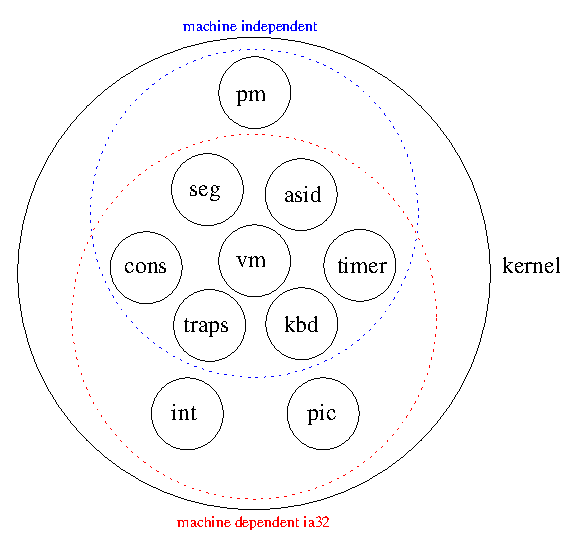
\includegraphics{figures/visualisation.eps}}
\end{figure}

Les modifications que nous pouvons observ\'ees sont les suivantes.

\subsection{Asid}

\paragraph{}

La gestion des identifiants d'espaces d'adressage contiendra d\'esormais
une partie ``machine independent'' et une partie ``machine dependent''.

\paragraph{}

En effet, lors de la r\'eservation/cr\'eation d'un espace d'adressage,
le kernel se charge d'allouer une structure de donn\'ees pour sa gestion
mais se chargera \'egalement d\'esormais de l'initialisation de ces
structures ainsi que de l'installation et l'initialisation des structures
de donn\'ees hardware.

\paragraph{}

Pour ces raisons, la gestion des espaces d'adressages contiendra une partie
``machine dependent'' qui se chargera de la gestion des ces parties hardware.

\section{Vm}

Comme vous pouvez le constater sur le sch\'ema, la gestion de la m\'emoire
virtuelle contient une partie ``machine independent'' qui a pour r\^ole
de g\'erer les structures de donn\'ees software d\'ecrivant les espaces
d'adressage virtuels propre \`a chaque processus.

\paragraph{}

La partie ``machine dependent'', elle, se contente de g\'erer les structures
de donn\'ees hardware, dans le cas d'Intel les page directories et page
tables.

\subsection{Bonus}

\paragraph{}

Nous vous proposons en bonus le d\'eveloppement de la fonction malloc
pour pouvoir allouer de la m\'emoire avec une granularit\'e accrue.

\paragraph{}

Il vous sera demand\'e de construire votre malloc intelligemment de sorte
que le m\^eme code puisse fonctionner pour un espace d'adressage diff\'erent,
c'est \`a dire pour un processus.

\end{document}

